\documentclass[a4paper]{article}
\usepackage[
	pdftex,
	colorlinks=true,
	bookmarksnumbered=true,
	bookmarksopen=true,
	bookmarksopenlevel=3,
	pdfstartview=FitP,
	urlcolor=blue,
]{hyperref}
\pdfinfo{
	/Title(Esercitazione di Laboratorio: Amplificatori operazionali con retroazione)
	/Author(Coa Giulio, Licastro Dario, Montano Alessandra)
}
\usepackage[italian]{babel}
\usepackage{amsmath,enumerate,enumitem,geometry,graphicx,mdsymbol,stmaryrd,subcaption,titling}
\graphicspath{{./Image/}}
\renewcommand\maketitlehooka{
	\null
	\mbox{}
	\vfill
}
\renewcommand\maketitlehookd{
	\vfill
	\null
}
\title{
	\begin{center}
		Esercitazione di Laboratorio:
	\end{center}
	\newline
	\begin{center}
		Amplificatori operazionali con retroazione
	\end{center}
}
\author{
	Coa Giulio
	\and
	Licastro Dario
	\and
	Montano Alessandra
}
\begin{document}
	%-----------------------------------------------------------------------------
	%  TITLE
	%-----------------------------------------------------------------------------
	\begin{titlingpage}
		\maketitle
	\end{titlingpage}
	\newpage
	%-----------------------------------------------------------------------------
	%  PURPOSE OF THE EXPERIENCE
	%-----------------------------------------------------------------------------
	\section{Scopo dell'esperienza}
	Gli scopi di questa esercitazione sono:
	\begin{itemize}
		\item Analizzare il comportamento e misurare i parametri di amplificatori reazionati.
		\item Verificare alcune deviazioni rispetto al comportamento previsto con i modelli ideali.
	\end{itemize}
	%-----------------------------------------------------------------------------
	%  INSTRUMENTATION USED
	%-----------------------------------------------------------------------------
	\section{Strumentazione utilizzata}
	La strumentazione usata durante l'esercitazione è:
	\begin{center}
		\begin{tabular}{ |c|c|c| }
			\hline
			\multirow{\textbf{Strumento}}	 & \textbf{Marca e Modello} & \textbf{Caratteristiche} \\
			\hline
			\multirow{Oscilloscopio}		 & Rigol DS1054Z			& 4 canali, \\
											 &							& $ B = 50 \, \mathrm{MHz} $, \\
											 &							& $ f_{\mathrm{c}} = 1 \, \mathrm{G\frac{Sa}{s}} $, \\
											 &							& $ R_{\mathrm{i}} = 1 \, \mathrm{M\Omega} $, \\
											 &							& $ C_{\mathrm{i}} = 13 \, \mathrm{pF} $, \\
											 &							& $ 12 \, \mathrm{Mbps} $ di profondità di memoria \\
			\multirow{Generatore di segnali} & Rigol DG1022				& 2 canali, \\
											 &							& $ f_{\mathrm{uscita}} = 20 \, \mathrm{MHz} $, \\
											 &							& $ Z_{\mathrm{uscita}} = 50 \, \mathrm{\Omega} $ \\
			\multirow{Alimentatore in DC}	 & Rigol DP832				& 3 canali \\
			\multirow{Scheda premontata}	 & A3						& \\
			\multirow{Cavi coassiali}		 &							& Capacità dell'ordine dei $ 80 \div 100 \, \mathrm{p\frac{F}{m}} $ \\
			\multirow{Connettori}			 &							& \\
			\hline
		\end{tabular}
	\end{center}
	%-----------------------------------------------------------------------------
	%  THEORETICAL PREMISES
	%-----------------------------------------------------------------------------
	\section{Premesse teoriche}
		\subsection{Incertezza sulla misura dell'oscilloscopio}
			La misura del valore di un segnale tramite l’oscilloscopio (sia esso l'ampiezza, la frequenza, il periodo, etc.) presenta un'incertezza che dipende, principalmente, da due fattori:
			\begin{itemize}
				\item l’incertezza strumentale introdotta dall’oscilloscopio (ricavabile dal manuale).
				\item l’incertezza di lettura dovuta all’errore del posizionamento dei cursori.
			\end{itemize}
			Quest’ultima incertezza deriva dal fatto che il segnale visualizzato non ha uno spessore nullo sullo schermo.
		\subsection{Amplificatore}
			Un amplificatore è un doppio bipolo unidirezionale caratterizzato dalla seguente relazione
			\begin{center}
				$ y(t) = A \cdot x(t) $
			\end{center}
			\newline
			Dove $ A $ è detto guadagno dell'amplifiatore.
			\begin{figure}[h!]
				\centering
				\begin{subfigure}{0.4\textwidth}
					\centering
					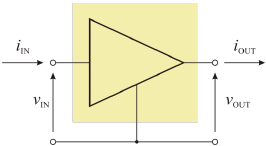
\includegraphics[scale=0.7]{amplificatore}
					\caption{Amplificatore.}
				\end{subfigure}
				\begin{subfigure}{0.4\textwidth}
					\centering
					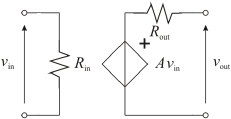
\includegraphics[scale=0.7]{amplificatoreCircuito}
					\caption{Circuito equivalente ad un amplificatore.}
				\end{subfigure}
				\label{fig:amplificatore}
			\end{figure}
			\newpage
			In base al tipo di segnale in ingresso e in uscita, possiamo distinguere quattro tipi di amplifiatori:
			\begin{itemize}
				\item Amplificatore di Tensione.
				\item Amplificatore di Transconduttanza.
				\item Amplificatore di Transresistenza.
				\item Amplificatore di Corrente.
			\end{itemize}
			\subsubsection{Amplificatore operazionale}
				L'amplificatore operazionale è un amplificatore differenziale, ovvero amplifica la differenza delle tensioni ai suoi capi, che presenta un'amplificazione $ A_{\mathrm{d}} $ idealmente infinita.
				\begin{equation*}
					\begin{split}
						A_{\mathrm{d}} &= \frac{v_{\mathrm{out}}}{v_{\mathrm{d}}} = \\
									   &= \frac{v_{\mathrm{out}}}{v^{+} - v^{-}}
					\end{split}
				\end{equation*}
				\begin{figure}[h!]
					\centering
					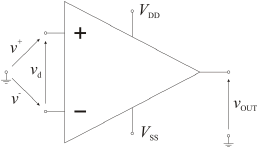
\includegraphics[scale=0.7]{amplificatoreOperazionale}
					\caption{Amplificatore operazionale.}
					\label{fig:amplificatoreOperazionale}
				\end{figure}
			\subsubsection{Amplificatore invertente}
				L'amplificatore invertente è un derivato dell'amplificatore di transresistenza che fornisce, in uscita, un segnale proporzionale al segnale in ingresso ma che presenta fase invertita rispetto ad esso; è caratterizzato dalle seguenti relazioni
				\begin{equation*}
				\begin{split}
					v_{\mathrm{out}} &= A_{\mathrm{v}} \cdot v_{\mathrm{in}} = \\
									 &= -\frac{R_{2}}{R_{1}} \cdot v_{\mathrm{in}}
				\end{split}
				\end{equation*}
				\begin{center}
					$ R_{\mathrm{in}} = R_{1} $
				\end{center}
				\newline
				\begin{center}
					$ R_{\mathrm{out}} = 0 $
				\end{center}
				\newline
				\begin{figure}[h!]
					\centering
					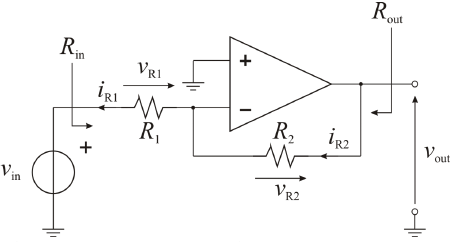
\includegraphics[scale=0.7]{amplificatoreInvertente}
					\caption{Amplificatore invertente.}
					\label{fig:amplificatoreInvertente}
				\end{figure}
				\newline
				\begin{scriptsize}
					\textbf{N.B.} $ R_{\mathrm{in}} $ non è necessariamente elevata. 
				\end{scriptsize}
			\subsubsection{Amplificatore differenziale}
				L'amplificatore differenziale è un amplificatore che fornisce, in uscita, un segnale proporzionale alla differenza rispetto ai segnali in ingresso; esso caratterizzato dalle seguenti relazioni
				\begin{center}
					$ R_{\mathrm{in, v^{+}}} = R_{\mathrm{a}} + R_{\mathrm{b}} $
				\end{center}
				\newline
				\begin{center}
					$ R_{\mathrm{in, v^{-}}} = R_{\mathrm{b}}^{'} $
				\end{center}
				\newline
				\begin{center}
					$ R_{\mathrm{out}} = 0 $
				\end{center}
				\newline
				\begin{center}
					$ \frac{R_{\mathrm{a}}^{'}}{R_{\mathrm{b}}^{'}} = \frac{R_{\mathrm{a}}}{R_{\mathrm{b}}} \cdot (1 + \epsilon) $
				\end{center}
				\newline
				\begin{equation*}
					\begin{split}
						v_{\mathrm{out}} &= A_{\mathrm{diff}} \cdot v_{\mathrm{d}} - A_{\mathrm{cm}} \cdot v_{\mathrm{cm}} = \\
										 &= (\frac{R_{\mathrm{a}}}{R_{\mathrm{b}}} - \frac{R_{\mathrm{a}}}{R_{\mathrm{a}} + R_{\mathrm{b}}} \cdot \frac{\epsilon}{2}) \cdot v_{\mathrm{d}} - \frac{R_{\mathrm{a}}}{R_{\mathrm{a}} + R_{\mathrm{b}}} \cdot \epsilon \cdot v_{\mathrm{cm}} = \\
										 &\approx \frac{R_{\mathrm{a}}}{R_{\mathrm{b}}} \cdot v_{\mathrm{d}} - \frac{R_{\mathrm{a}}}{R_{\mathrm{a}} + R_{\mathrm{b}}} \cdot \epsilon \cdot v_{\mathrm{cm}}
					\end{split}
				\end{equation*}
				\begin{center}
					$ \mathrm{CMRR} = \frac{A_{\mathrm{diff}}}{A_{\mathrm{cm}}} \approx \frac{1}{\epsilon} \cdot (1 + A_{\mathrm{diff}}) $
				\end{center}
				\newline
				Dove $ \mathrm{CMRR} $ è il Common-Mode Rejection Ratio, $ A_{\mathrm{diff}} $ è l'amplificazione differenziale e $ A_{\mathrm{cm}} $ è l'amplificazione di modo comune.
				\begin{figure}[h!]
					\centering
					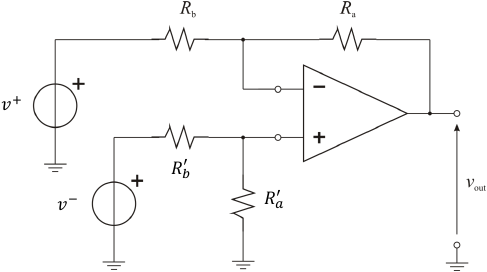
\includegraphics[scale=0.7]{amplificatoreDifferenziale}
					\caption{Amplificatore differenziale.}
					\label{fig:amplificatoreDifferenziale}
				\end{figure}
				\newpage
	%-----------------------------------------------------------------------------
	%  LABORATORY EXPERIENCE
	%-----------------------------------------------------------------------------
	\section{Esperienza in laboratorio}
		\subsection{Amplificatore non invertente}
			Abbiamo realizzato il circuito richiesto, collegando il modulo A3-1:
			\begin{itemize}
				\item Il generatore di segnali al connettore coassiale J15.
				\item L'alimentatore duale viene connesso, in modalità tracking, al morsetto Val.
				\item L'oscilloscopio, tramite due cavi coassiali BNC-coccodrillo, all'ingresso e all'uscita del circuito, rispettivamente gli ancoraggi J3 e J7 (massa) e J2 e J8 (massa).
			\end{itemize}
			E posizionando gli interruttori seguendo la seguente tabella
			\begin{center}
				\begin{tabular}{ |c|c|c| }
					\hline
					\multirow{\textbf{Interruttore}} & \textbf{Posizione} & \textbf{Note} \\
					\hline
					\multirow{S1}		     		 & 1				  & aperto \\
					\multirow{S2}		     		 & 2				  & chiuso \\
					\multirow{S4}		     		 & 2				  & chiuso \\
					\multirow{S5}		     		 & 1				  & aperto \\
					\multirow{S6}		     		 & 1				  & aperto \\
					\hline
				\end{tabular}
			\end{center}
			Infine, abbiamo impostato il generatore di segnali, in modo da visualizzare un segnale sinusoidale con $ V_{\mathrm{pp}} $ pari ad $ 1 \, \mathrm{V} $ e frequenza pari a $ 2 \, \mathrm{kHz} $, e proceduto con la misurazione di $ V_{\mathrm{i}} $ e $ V_{\mathrm{u}} $, tramite l'uso dell'oscilloscopio.
		\subsection{Amplificatore invertente}
			Abbiamo realizzato il circuito richiesto, collegando il modulo A3-2:
			\begin{itemize}
				\item Il generatore di segnali al connettore coassiale J16.
				\item L'oscilloscopio, tramite due cavi coassiali BNC-coccodrillo, all'ingresso e all'uscita del circuito, rispettivamente gli ancoraggi J9 e J14 (massa) e J11 e J13 (massa).
			\end{itemize}
			E posizionando gli interruttori seguendo la seguente tabella
			\begin{center}
				\begin{tabular}{ |c|c|c| }
					\hline
					\multirow{\textbf{Interruttore}} & \textbf{Posizione} & \textbf{Note} \\
					\hline
					\multirow{S8}		     		 & 1				  & aperto \\
					\multirow{S9}		     		 & 1				  & aperto \\
					\multirow{S10}		     		 & 2				  & chiuso \\
					\multirow{S11}		     		 & 1				  & aperto \\
					\multirow{S12}		     		 & 1				  & aperto \\
					\multirow{S13}		     		 & 1				  & $ R_{11} $ non inserita \\
					\multirow{S14}		     		 & 1				  & $ R_{12} $ non inserita \\
					\hline
				\end{tabular}
			\end{center}
			Successivamente, abbiamo impostato il generatore di segnali, in modo da visualizzare un segnale triangolare con $ V_{\mathrm{pp}} $ pari ad $ 2 \, \mathrm{V} $ e frequenza pari a $ 300 \, \mathrm{Hz} $, e proceduto con la misurazione di $ V_{\mathrm{i}} $ e $ V_{\mathrm{u}} $, tramite l'uso dell'oscilloscopio.
			\newline
			Infine, abbiamo verificato che la tensione sui morsetti dell'amplificatore fosse nulla o prossima allo zero ed abbiamo proceduto ad aumentare l'ampiezza del segnale al fine di ottenere il presentarsi del fenomeno di clipping.
			\begin{figure}[h!]
				\centering
				\begin{subfigure}{0.4\textwidth}
					\centering
					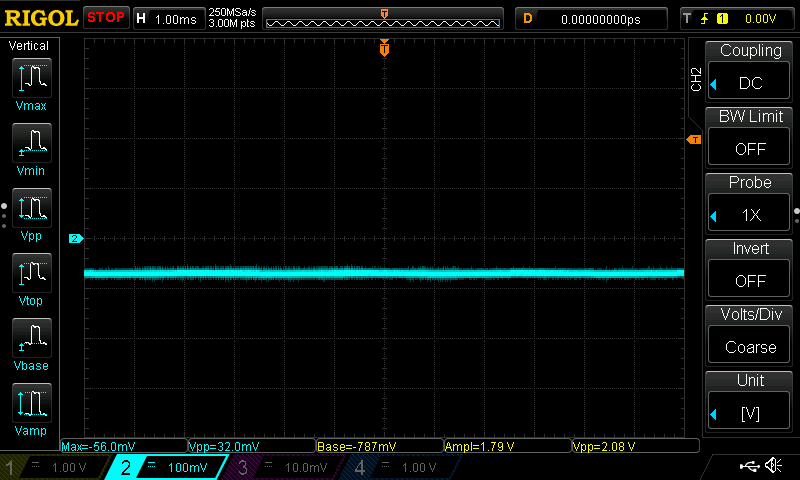
\includegraphics[scale=0.2]{tensioneMorsettoNonInvertente}
					\caption{Verifica della tensione al morsetto non-invertente.}
				\end{subfigure}
				\begin{subfigure}{0.4\textwidth}
					\centering
					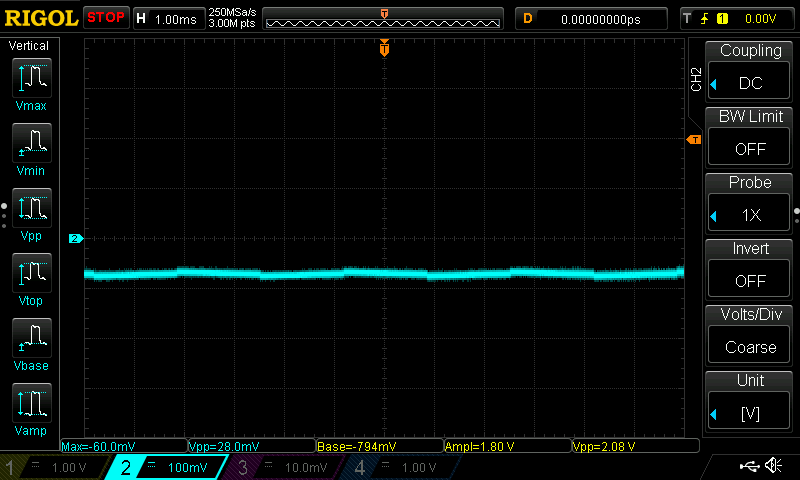
\includegraphics[scale=0.2]{tensioneMorsettoInvertente}
					\caption{Verifica della tensione al morsetto invertente.}
				\end{subfigure}
				\begin{subfigure}{0.7\textwidth}
					\centering
					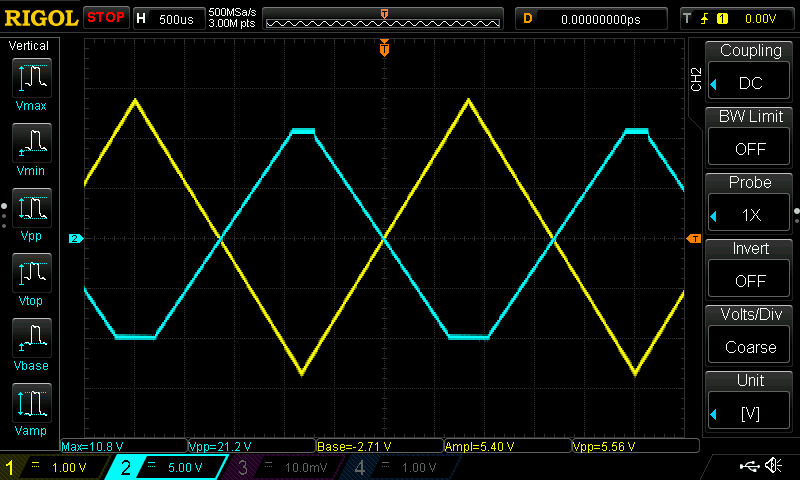
\includegraphics[scale=0.3]{clipping}
					\caption{Verifica del fenomeno di clipping ($ V_{\mathrm{pp}} = 5.5 \, \mathrm{V} $).}
				\end{subfigure}
				\label{fig:punto2.2.3}
			\end{figure}
		\subsection{Amplificatore differenziale}
			Abbiamo realizzato il circuito richiesto, posizionando gli interruttori seguendo la seguente tabella
			\begin{center}
				\begin{tabular}{ |c|c|c| }
					\hline
					\multirow{\textbf{Interruttore}} & \textbf{Posizione} & \textbf{Note} \\
					\hline
					\multirow{S12}		     		 & 2				  & chiuso \\
					\multirow{S13}		     		 & 1				  & $ R_{11} $ non inserita \\
					\multirow{S14}		     		 & 1				  & $ R_{12} $ non inserita \\
					\hline
				\end{tabular}
			\end{center}
			Successivamente, abbiamo impostato il generatore di segnali, in modo da visualizzare un segnale sinusoidale con $ V_{\mathrm{pp}} $ pari ad $ 1.6 \, \mathrm{V} $ e frequenza pari a $ 200 \, \mathrm{Hz} $, e proceduto con la misurazione di $ V_{\mathrm{i}} $ e $ V_{\mathrm{u}} $, tramite l'uso dell'oscilloscopio, per le varie configurazioni.
		\subsection{Amplificatore AC/DC}
			Abbiamo realizzato il circuito richiesto, collegando il modulo A3-1:
			\begin{itemize}
				\item Il generatore di segnali al connettore coassiale J15.
				\item L'oscilloscopio, tramite due cavi coassiali BNC-coccodrillo, all'ingresso e all'uscita del circuito, rispettivamente gli ancoraggi J3 e J7 (massa), J2 e J8 (massa).
			\end{itemize}
			E, dopo aver posizionato gli interruttori seguendo la seguente tabella,
			\begin{center}
				\begin{tabular}{ |c|c|c| }
					\hline
					\multirow{\textbf{Interruttore}} & \textbf{Posizione} & \textbf{Note} \\
					\hline
					\multirow{S3}		     		 & 2				  & chiuso \\
					\multirow{S5}		     		 & 2				  & chiuso \\
					\multirow{S6}		     		 & 1				  & aperto \\
					\hline
				\end{tabular}
			\end{center}
			Poi, prima di procedere con l'esperienza, abbiamo impostato il generatore di segnali, in modo da visualizzare un segnale sinusoidale con $ V_{\mathrm{pp}} $ pari ad $ 1.6 \, \mathrm{V} $ e frequenza pari a $ 10 \, \mathrm{kHz} $.
			\newline
			Infine, abbiamo valutato, nel dominio di Laplace, il circuito nelle varie configurazioni.
			\begin{enumerate}[label=\alph*.]
				\item \ 
					\newline
					Successivamente, abbiamo osservato come, al crescere della frequenza, il segnale venga distorto a causa della limitazione di Slew Rate.
					\begin{figure}[h!]
						\centering
						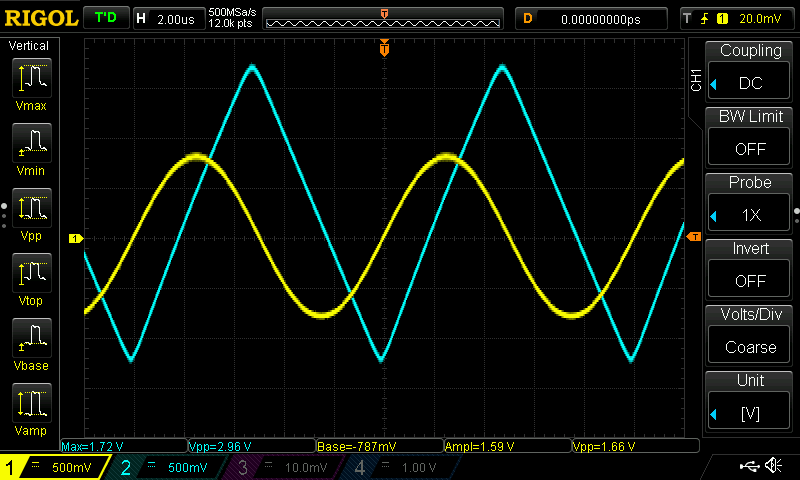
\includegraphics[scale=0.4]{slewRate}
						\caption{Verifica della limitazione di Slew Rate.}
						\label{fig:slewRate}
					\end{figure}
					\newline
					Di conseguenza, abbiamo determinato sperimentalmente quale fosse la tensione per cui la limitazione di Slew Rate fosse rispettata ed abbiamo proceduto al ridurre l'ampiezza $ V_{\mathrm{pp}} $ fino a tale valore, passando da $ 1.6 \, \mathrm{V} $ a $ 300 \, \mathrm{mV} $.
					\begin{figure}[h!]
						\centering
						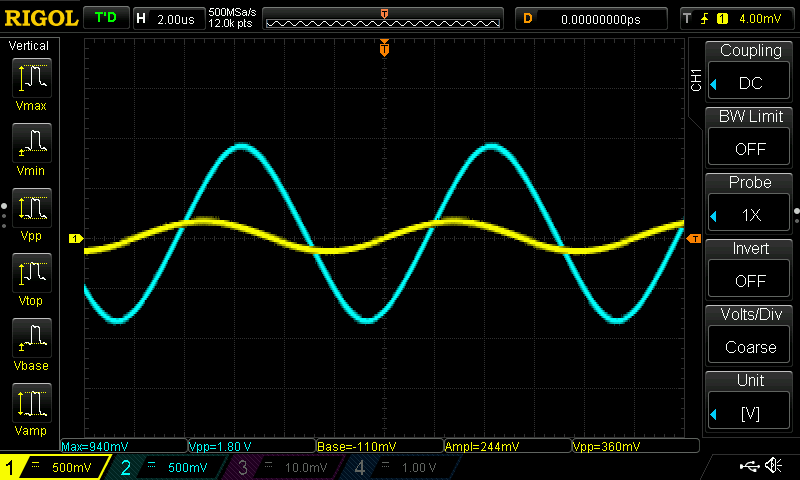
\includegraphics[scale=0.4]{segnaleCorrettoSlewRate}
						\caption{Ingresso ed uscita dell'amplificatore alla frequenza di $ 100 \, \mathrm{kHz} $.}
						\label{fig:segnaleCorrettoSlewRate}
					\end{figure}
					\newpage
					A questo punto abbiamo proceduto con la misurazione di $ V_{\mathrm{i}} $ e $ V_{\mathrm{u}} $, tramite l'uso dell'oscilloscopio, alle varie frequenze in esame.
				\item \label{item:b} \ 
					\newline
					Al fine di determinare la frequenza di taglio, abbiamo determinato il valore di $ V_{\mathrm{u}} $ una volta attenuato di $ 3 \, \mathrm{dB} $ e abbiamo variato la frequenza affinchè il valore di $ V_{\mathrm{u}} $ si avvicinasse il più possibile al valore calcolato.
				\item \ 
					\newline
					Al fine di verificare che l'amplificatore amplificasse eventuali offset del segnale, abbiamo applicato, dapprima, un offset di $ 140 \, \mathrm{mV} $ e, successivamente, un offset di $ 180 \, \mathrm{mV} $, riscontrando un'amplificazione di un fattore $ A_{\mathrm{v}} $ del suddetto.
					\newline
					Sono stati mantenuti valori piccoli per gli offset di modo da evitare errate visualizzazioni del segnale.
					\begin{figure}[h!]
						\centering
						\begin{subfigure}{0.4\textwidth}
							\centering
							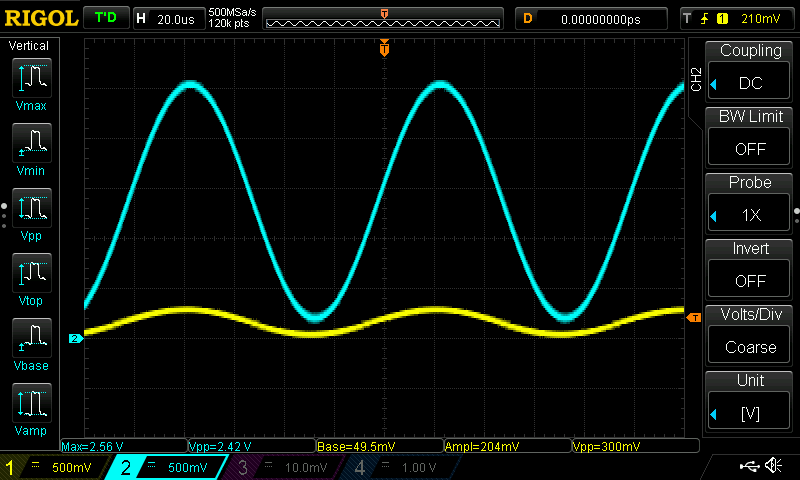
\includegraphics[scale=0.2]{offset140}
							\caption{Segnale con un offset di $ 140 \, \mathrm{mV} $.}
						\end{subfigure}
						\begin{subfigure}{0.4\textwidth}
							\centering
							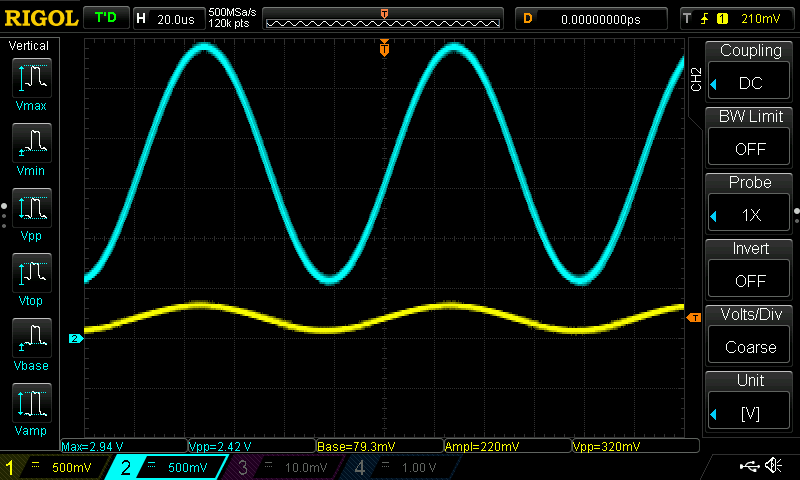
\includegraphics[scale=0.2]{offset180}
							\caption{Segnale con un offset di $ 180 \, \mathrm{mV} $.}
						\end{subfigure}
						\label{fig:punto2.4.3.c}
					\end{figure}
				\item \ 
					\newline
					\textbf{N.B.} Il condensatore $ C_{3} $ preso in esame ha un valore di $ 15 \, \mathrm{pF} $ e non di $ 10 \, \mathrm{nF} $ come riportato nel testo dell'esercitazione; ciò ha portato ad un'esperienza che si discosta da quella che era stata pensata per l'esercitazione.
					\newline
					\newline
					Abbiamo commutato lo switch S1, inserendo il condensatore $ C_{3} $ nel circuito, ed abbiamo ripetuto la procedura al punto~\ref{item:b} al fine di determinare la nuova frequenza di taglio.
					\newline
					Infine, abbiamo determinato il guadagno in continua dell'amplificatore tramite l'applicazione di due offset.
					\begin{figure}[h!]
						\centering
						\begin{subfigure}{0.4\textwidth}
							\centering
							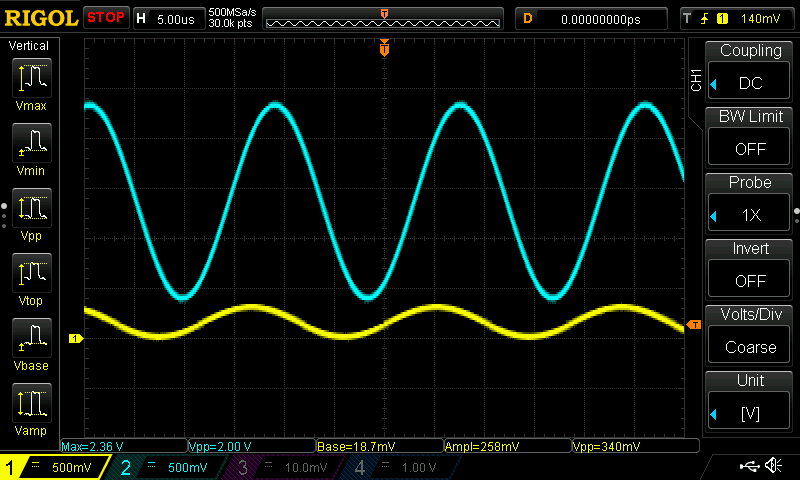
\includegraphics[scale=0.2]{offset140C3}
							\caption{Segnale con un offset di $ 140 \, \mathrm{mV} $.}
						\end{subfigure}
						\begin{subfigure}{0.4\textwidth}
							\centering
							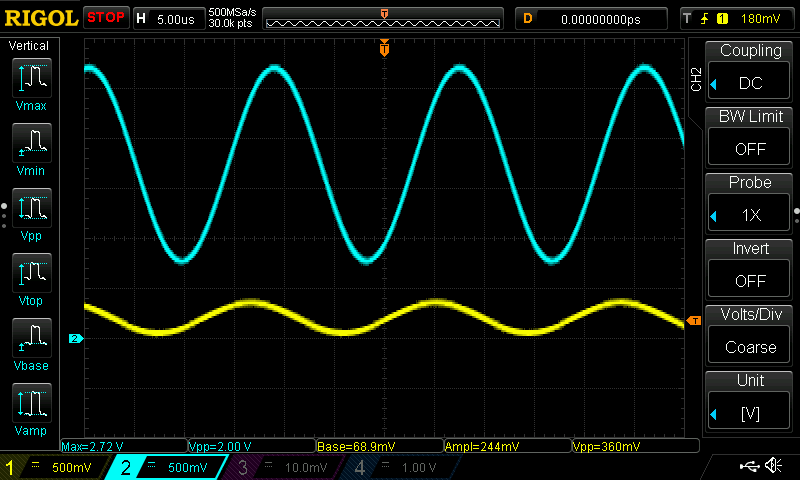
\includegraphics[scale=0.2]{offset180C3}
							\caption{Segnale con un offset di $ 180 \, \mathrm{mV} $.}
						\end{subfigure}
						\label{fig:punto2.4.3.d}
					\end{figure}
				\item \ 
					\newline
					Abbiamo commutato lo switch S2, inserendo il condensatore $ C_{4} $ nel circuito, ed abbiamo ripetuto la procedura al punto~\ref{item:b} al fine di determinare la nuova frequenza di taglio.
					\newline
					Inoltre, si è verificato come l'offset in ingresso non venisse amplificato in uscita.
				\item \ 
					\newline
					Abbiamo commutato lo switch S4, inserendo il condensatore $ C_{5} $ nel circuito, ed abbiamo ripetuto la procedura al punto~\ref{item:b} al fine di determinare la nuova frequenza di taglio.
					\newline
					Inoltre, si è verificato come l'offset in ingresso venisse annullato in uscita.
			\end{enumerate}
	%-----------------------------------------------------------------------------
	%  RESULTS
	%-----------------------------------------------------------------------------
	\section{Risultati}
		\subsection{Amplificatore non invertente}
			Dai calcoli abbiamo ricavato l'amplificazione 
			\begin{equation*}
				\begin{split}
					A_{\mathrm{v}} &= \frac{A_{\mathrm{d}}}{1 + \beta \cdot A_{\mathrm{d}}} = \\
								   &= \frac{A_{\mathrm{d}}}{1 + \frac{R_{2}}{R_{1} + R_{2}} \cdot A_{\mathrm{d}}} = \\
								   &= \frac{200k}{1 + \frac{12k}{100k + 12k} \cdot 200k} = \\
								   &= 9.33
					\end{split}
			\end{equation*}
			\begin{equation*}
				\begin{split}
					R_{\mathrm{in}} &= (R_{\mathrm{id}} + R_{3} + (R_{1} + R_{\mathrm{o}}) \parallel R_{2}) \cdot (1 + A_{\mathrm{d}} \cdot \frac{R_{2} \parallel (R_{\mathrm{id}} + R_{3}) + R_{\mathrm{o}}}{R_{2} \parallel (R_{\mathrm{id}} + R_{3}) + R_{\mathrm{o}} + R_{1}}) = \\
									&= (1M + 4.7k + (100k + 100) \parallel 12k) \cdot (1 + 200k \cdot \frac{12k \parallel (1M + 4.7k) + 100}{12k \parallel (1M + 4.7k) + 100 + 100k}) = \\
									&= 21.7 \, \mathrm{G\Omega}
				\end{split}
			\end{equation*}
			\begin{equation*}
				\begin{split}
					R_{\mathrm{out}} &= \frac{R_{\mathrm{o}}}{1 + \beta \cdot A_{\mathrm{d}}} \parallel (R_{1} + R_{2}) = \\
									 &= \frac{R_{\mathrm{o}}}{1 + \frac{R_{2}}{R_{1} + R_{2}} \cdot A_{\mathrm{d}}} \parallel (R_{1} + R_{2}) = \\
									 &= \frac{100}{1 + \frac{12k}{100k + 12k} \cdot 200k} \parallel (100k + 12k) = \\
									 &= 4.67 \, \mathrm{m\Omega}
				\end{split}
			\end{equation*}
			\begin{center}
				\begin{tabular}{ |c|c|c|c|c| }
					\hline
					\multirow{\textbf{S3}} & \textbf{S7} & \textbf{$ V_{\mathrm{i}} $ [$ \mathrm{V} $]} & \textbf{$ V_{\mathrm{u}} $ [$ \mathrm{V} $]} & \textbf{$ A_{\mathrm{v}} $} \\
					\hline
					\multirow{1}		   & 1			 & $ 1.08 $ 									& $ 9.80 $ 									   & $ 9.07 $ \\
					\multirow{1}		   & 2			 & $ 1.08 $ 									& $ 9.80 $ 									   & $ 9.07 $ \\
					\multirow{2}		   & 1			 & $ 1.08 $ 									& $ 10.0 $ 									   & $ 9.26 $ \\
					\multirow{2}		   & 2			 & $ 1.08 $ 									& $ 10.0 $ 									   & $ 9.26 $ \\
					\hline
				\end{tabular}
			\end{center}
			Notiamo che i valori di $ A_{\mathrm{v}} $ ottenuti dalle misurazioni sono leggermente più bassi del valore teorico; tale la differenza è piccola e, pertanto, trascurabile.
			\newline
			Sfruttando il partitore di tensione formatosi all'ingresso dell'amplifiatore quando la resistenza $ R_{3} $ è inserita, possiamo scrivere
			\begin{equation*}
				\begin{split}
					w &= \frac{v_{\mathrm{out,R_{3}}}}{v_{\mathrm{out}}} = \\
					  &= 0.98
				\end{split}
			\end{equation*}
			\begin{equation*}
				\begin{split}
					w &= \frac{v_{\mathrm{out,R_{3}}}}{v_{\mathrm{out}}} = \\
					  &= \frac{A_{\mathrm{v}} \cdot V_{\mathrm{i,R_{3}}}}{A_{\mathrm{v}} \cdot V_{\mathrm{i}}} = \\
					  &= \frac{V_{\mathrm{i,R_{3}}}}{V_{\mathrm{i}}} = \\
					  &= \frac{v_{\mathrm{s}} \cdot \frac{R_{\mathrm{i}}}{R_{3} + R_{\mathrm{i}}}}{v_{\mathrm{s}}} = \\
					  &= \frac{R_{\mathrm{i}}}{R_{3} + R_{\mathrm{i}}}
				\end{split}
			\end{equation*}
			Da cui
			\begin{equation*}
					\begin{split}
						R_{\mathrm{i}} &= w \cdot R_{3} \cdot \frac{1}{1 - w} = \\
									   &= 0.98 \cdot 4.7k \cdot \frac{1}{1 - 0.98} = \\
									   &= 230 \, \mathrm{k\Omega}
					\end{split}
			\end{equation*}
			Il valore ottenuto ci conferma che la resistenza in ingresso è elevata e che, dato che le due tensioni misurate quando $ R_{5} $ è inserita sono uguali, il valore di $ R_{\mathrm{u}} $ è trascurabile.
		\subsection{Amplificatore invertente}
			Dai calcoli abbiamo ricavato che
			\begin{equation*}
				\begin{split}
					A_{\mathrm{v}} &= \frac{A_{\mathrm{d}}}{1 + \beta \cdot A_{\mathrm{d}}} = \\
								   &= \frac{A_{\mathrm{d}}}{1 -\frac{R_{9}}{R_{10}} \cdot A_{\mathrm{d}}} = \\
								   &= \frac{200k}{1 -\frac{22k}{100k} \cdot 200k} = \\
								   &= -4.55
				\end{split}
			\end{equation*}
			\begin{equation*}
				\begin{split}
					R_{\mathrm{in}} &= R_{9} + \frac{R_{\mathrm{o}} + R_{10}}{1 + A_{\mathrm{d}}} = \\
									&= 22k + \frac{100 + 100k}{1 + 200k} = \\
									&\approx 22 \, \mathrm{k\Omega}
				\end{split}
			\end{equation*}
			\begin{equation*}
				\begin{split}
					R_{\mathrm{out}} &= \frac{R_{\mathrm{o}} + R_{9} + R_{10}}{R_{\mathrm{o}} + R_{9} \cdot (1 + A_{\mathrm{d}}) + R_{10}} \cdot [R_{\mathrm{o}} \parallel (R_{9} + R_{10})] = \\
									 &= \frac{100 + 22k + 100k}{100 + 22k \cdot (1 + 200k) + 100k} \cdot [100 \parallel (22k + 100k)] = \\
									 &= 2.77 \, \mathrm{m\Omega}
				\end{split}
			\end{equation*}
			\begin{center}
				\begin{tabular}{ |c|c|c| }
					\hline
					\multirow{\textbf{$ V_{\mathrm{i}} $ [$ \mathrm{V} $]}} & \textbf{$ V_{\mathrm{u}} $ [$ \mathrm{V} $]} & \textbf{$ A_{\mathrm{v}} $} \\
					\hline
					\multirow{$ 2.16 $} 									& $ 9.20 $ 									   & $ 4.26 $ \\
					\hline
				\end{tabular}
			\end{center}
			Notiamo che il valore di $ A_{\mathrm{v}} $ ottenuto dalle misurazioni è leggermente più basso del valore teorico; tale la differenza è piccola e, pertanto, trascurabile. Inoltre, esso presenta segno positivo poichè l’oscilloscopio tiene in considerazione la differenza di fase di $ 180 $\textdegree \ tra l'ingresso e l'uscita.
		\subsection{Amplificatore differenziale}
			Chiudendo lo switch S8, creiamo una maglia priva di resistenze dove, per l'appunto, la tensione sul morsetto non-invertente è pari a quella sul morsetto invertente ($ V_{2} = V_{\mathrm{i}} $); a causa di ciò, la differenza tra le due tensioni è nulla ed il guadagno dell'amplificatore differenziale sarà unitario, ovvero non vi sarà una variazione del segnale.
			\begin{equation*}
				\begin{split}
					A_{\mathrm{v, S8}} &= 1 + \frac{R_{10}}{R_{9}} - \frac{R_{10}}{R_{9}} = \\
									   &= 1 + \frac{100k}{22k} - \frac{100k}{22k} = \\
									   &= 1
				\end{split}
			\end{equation*}
			Chiudendo lo switch S9, creiamo una maglia in cui è presente la resistenza $ R_{6} $; a causa di ciò, si avrà una diminuzione della tensione sul morsetto non-invertente rispetto alla tensione sul morsetto invertente ($ V_{2} = \frac{2}{3} \cdot V_{\mathrm{i}} $).
			\begin{equation*}
				\begin{split}
					A_{\mathrm{v, S9}} &= \frac{2}{3} \cdot (1 + \frac{R_{10}}{R_{9}}) - \frac{R_{10}}{R_{9}} = \\
									   &= \frac{2}{3} \cdot (1 + \frac{100k}{22k}) - \frac{100k}{22k} = \\
									   &= -0.85
				\end{split}
			\end{equation*}
			Chiudendo lo switch S10, creiamo una maglia in cui è presente la resistenza $ R_{6} $ ed $ R_{7} $; a causa di ciò, si avrà una diminuzione della tensione sul morsetto non-invertente rispetto alla tensione sul morsetto invertente ($ V_{2} = \frac{1}{3} \cdot V_{\mathrm{i}} $) che porterà ad un incremento, in modulo, del guadagno dell'amplificatore, come riscontrabile dai calcoli.
			\begin{equation*}
				\begin{split}
					A_{\mathrm{v, S10}} &= \frac{1}{3} \cdot (1 + \frac{R_{10}}{R_{9}}) - \frac{R_{10}}{R_{9}} = \\
										&= \frac{1}{3} \cdot (1 + \frac{100k}{22k}) - \frac{100k}{22k} = \\
										&= -2.7
				\end{split}
			\end{equation*}
			Chiudendo lo switch S11, colleghiamo, direttamente, il morsetto non-invertente alla massa e, quindi, avremo che la tensione su di esso sarà nulla, rendendo l'amplificatore un amplificatore invertente.
			\begin{equation*}
				\begin{split}
					A_{\mathrm{v, S11}} &= - \frac{R_{10}}{R_{9}} = \\
										&= - \frac{100k}{22k} = \\
										&= -4.55
				\end{split}
			\end{equation*}
			\begin{center}
				\begin{tabular}{ |c|c|c|c|c|c|c| }
					\hline
					\multirow{\textbf{S8}} & \textbf{S9} & \textbf{S10} & \textbf{S11} & \textbf{$ V_{\mathrm{i}} $ [$ \mathrm{V} $]} & \textbf{$ V_{\mathrm{u}} $ [$ \mathrm{V} $]} & \textbf{$ A_{\mathrm{v}} $} \\
					\hline
					\multirow{2}		   & 1			 & 1			& 1			   & $ 1.66 $ 									  & $ 1.64 $ 								   & $ 0.99 $ \\
					\multirow{1}		   & 2			 & 1			& 1			   & $ 1.66 $ 									  & $ 1.40 $ 								   & $ 0.84 $ \\
					\multirow{1}		   & 1			 & 2			& 1			   & $ 1.64 $ 									  & $ 4.36 $ 								   & $ 2.66 $ \\
					\multirow{1}		   & 1			 & 1			& 2			   & $ 1.64 $ 									  & $ 7.32 $ 								   & $ 4.46 $ \\
					\hline
				\end{tabular}
			\end{center}
			Le misurazioni effettuate sono coerenti con i valori calcolati, infatti, abbiamo riscontrato differenze dell'ordine dei centesimi ($ 0.01 \div 0.09 $), ma tendenzialmente la differenza è molto minore.
			\newline
			\newline
			\begin{scriptsize}
				I calcoli effettuati sono stati svolti utilizzando il principio di sovrapposizione degli effetti. 
			\end{scriptsize}
		\subsection{Amplificatore AC/DC}
			\begin{enumerate}[label=\alph*.]
				\item \ 
					\newline
					\begin{center}
						\begin{tabular}{ |c|c|c|c| }
							\hline
							\multirow{\textbf{Frequenza}}	   & \textbf{$ V_{\mathrm{i}} $ [$ \mathrm{mV} $]} & \textbf{$ V_{\mathrm{u}} $ [$ \mathrm{V} $]} & \textbf{$ A_{\mathrm{v}} $} \\
							\hline
							\multirow{$ 100 \, \mathrm{Hz} $}  & $ 324 $ 									   & $ 2.96 $ 									  & $ 9.14 $ \\
							\multirow{$ 1 \, \mathrm{kHz} $}   & $ 324 $ 									   & $ 2.96 $ 									  & $ 9.14 $ \\
							\multirow{$ 10 \, \mathrm{kHz} $}  & $ 380 $ 									   & $ 2.88 $ 									  & $ 7.58 $ \\
							\multirow{$ 100 \, \mathrm{kHz} $} & $ 360 $ 									   & $ 1.80 $ 									  & $ 5.00 $ \\
							\hline
						\end{tabular}
					\end{center}
				\item \ 
					\newline
					\begin{center}
						$ 20 \log \frac{V_{\mathrm{u, f_{T}}}}{V_{\mathrm{u}}} = -3 $
					\end{center}
					\newline
					\begin{center}
						$ \frac{V_{\mathrm{u, f_{T}}}}{V_{\mathrm{u}}} = 10^{-\frac{3}{20}} $
					\end{center}
					\newline
					\begin{equation*}
						\begin{split}
							V_{\mathrm{u, f_{T}}} &= 10^{-\frac{3}{20}} \cdot V_{\mathrm{u}} = \\
												  &= 0.707 \cdot 2.88 = \\
												  &= 2.04 \, \mathrm{V}
						\end{split}
					\end{equation*}
					\begin{figure}[h!]
						\centering
						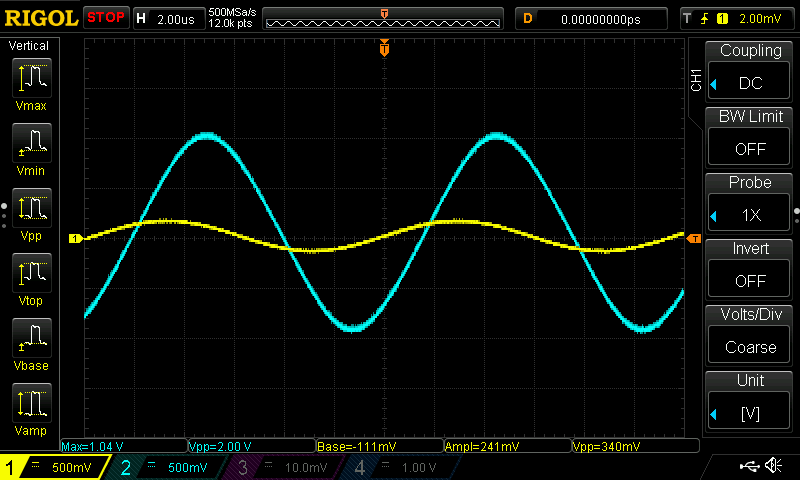
\includegraphics[scale=0.4]{frequenzaDiTaglio}
						\caption{Segnale alla frequenza di taglio ($ f = 86.08 \, \mathrm{kHz} $).}
						\label{fig:frequenzaDiTaglio}
					\end{figure}
				\item \ 
					\newline
					\textbf{N.B.} Il condensatore $ C_{3} $ preso in esame ha un valore di $ 15 \, \mathrm{pF} $ e non di $ 10 \, \mathrm{nF} $ come riportato nel testo dell'esercitazione; ciò ha portato ad un'esperienza che si discosta da quella che era stata pensata per l'esercitazione.
					\newline
					\newline
					\begin{figure}[h!]
						\centering
						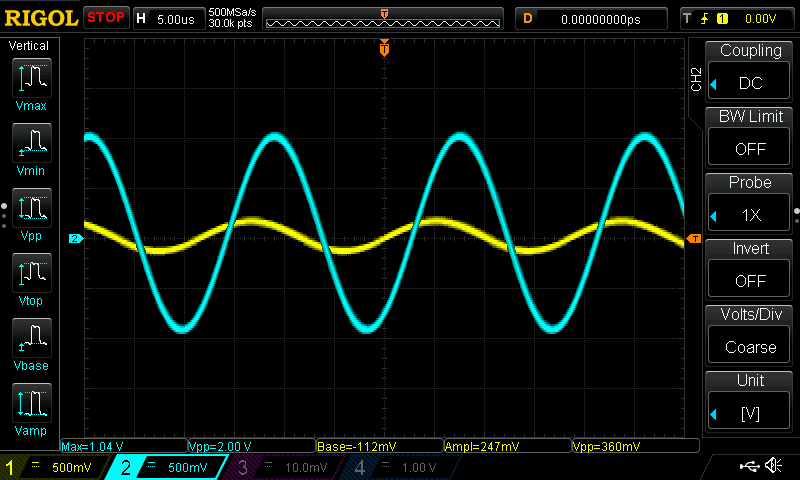
\includegraphics[scale=0.4]{frequenzaDiTaglioC3}
						\caption{Segnale alla frequenza di taglio ($ f = 54 \, \mathrm{kHz} $).}
						\label{fig:frequenzaDiTaglioC3}
					\end{figure}
					\newpage
					\begin{equation*}
						\begin{split}
							A_{\mathrm{v, DC}} &= \frac{V_{\mathrm{u, 140m}}}{V_{\mathrm{i, 140m}}} = \\
											   &= \frac{1.4}{140m} = \\
											   &= 10
						\end{split}
					\end{equation*}
					\begin{equation*}
						\begin{split}
							A_{\mathrm{v, DC}} &= \frac{V_{\mathrm{u, 180m}}}{V_{\mathrm{i, 180m}}} = \\
											   &= \frac{1.8}{180m} = \\
											   &= 10
						\end{split}
					\end{equation*}
				\item \ 
					\newline
					\newpage
					\begin{figure}[h!]
						\centering
						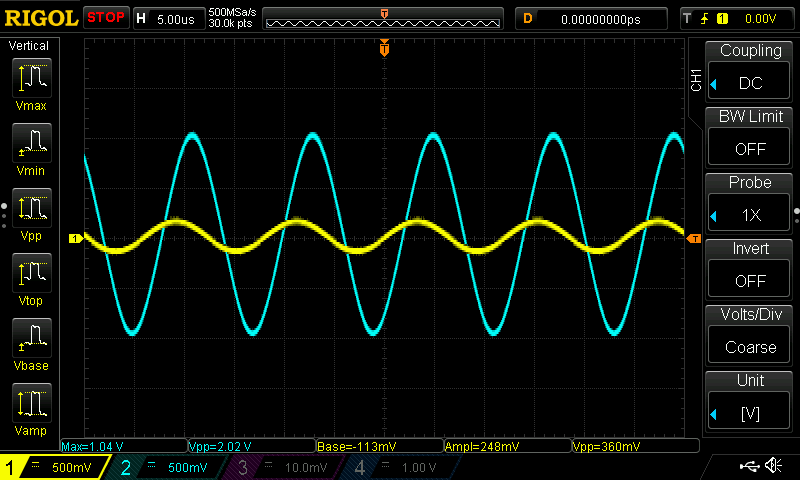
\includegraphics[scale=0.4]{frequenzaDiTaglioC4}
						\caption{Segnale alla frequenza di taglio ($ f = 83 \, \mathrm{kHz} $).}
						\label{fig:frequenzaDiTaglioC4}
					\end{figure}
					\newline
					\begin{equation*}
						\begin{split}
							A_{\mathrm{v, DC}} &= \frac{V_{\mathrm{u, 140m}}}{V_{\mathrm{i, 140m}}} = \\
											   &= \frac{140m}{140m} = \\
											   &= 1
						\end{split}
					\end{equation*}
					\begin{equation*}
						\begin{split}
							A_{\mathrm{v, DC}} &= \frac{V_{\mathrm{u, 180m}}}{V_{\mathrm{i, 180m}}} = \\
											   &= \frac{180m}{180m} = \\
											   &= 1
						\end{split}
					\end{equation*}
				\item \ 
					\newline
					\newpage
					\begin{figure}[h!]
						\centering
						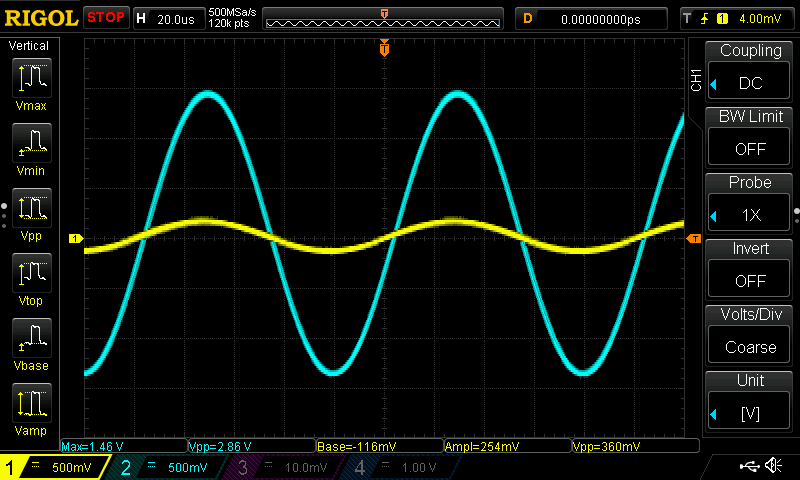
\includegraphics[scale=0.4]{frequenzaDiTaglioC5}
						\caption{Segnale alla frequenza di taglio ($ f = 84 \, \mathrm{kHz} $).}
						\label{fig:frequenzaDiTaglioC5}
					\end{figure}
					\newline
					\begin{equation*}
						\begin{split}
							A_{\mathrm{v, DC}} &= \frac{V_{\mathrm{u, 140m}}}{V_{\mathrm{i, 140m}}} = \\
											   &= \frac{0}{140m} = \\
											   &= 0
					\end{split}
					\end{equation*}
					\begin{equation*}
						\begin{split}
							A_{\mathrm{v, DC}} &= \frac{V_{\mathrm{u, 180m}}}{V_{\mathrm{i, 180m}}} = \\
											   &= \frac{0}{180m} = \\
											   &= 0
						\end{split}
					\end{equation*}
			\end{enumerate}
\end{document}